\documentclass{article}

\usepackage{listings} % Code samples
\usepackage{color} % Code markup styling
\usepackage{forest} % Directory graphics pt. 1
\usepackage{elocalloc} % Directory graphics pt. 2
\usepackage{dirtree} % Boring directory representation
\usepackage{graphicx} % For figures
\usepackage{wrapfig} % Wrapping text around figures
\usepackage[margin=1.81in]{geometry} % Adjust page margins
\usepackage{pgfplots} % Plot normal distribution

% Styling for directory graphics
\definecolor{aliceblue}{rgb}{0.94, 0.97, 1.0}

% Styling for code markup
\definecolor{codegreen}{rgb}{0,0.6,0}
\definecolor{codegray}{rgb}{0.5,0.5,0.5}
\definecolor{codepurple}{rgb}{0.58,0,0.82}
\definecolor{backcolour}{rgb}{0.95,0.95,0.92}

\lstdefinestyle{codestyle}{
	backgroundcolor=\color{backcolour},   
	commentstyle=\color{codegreen},
	keywordstyle=\color{magenta},
	numberstyle=\tiny\color{codegray},
	stringstyle=\color{codepurple},
	basicstyle=\footnotesize,
	breakatwhitespace=false,         
	breaklines=true,                 
	captionpos=b,                    
	keepspaces=true,                 
	numbers=left,                    
	numbersep=5pt,                  
	showspaces=false,                
	showstringspaces=false,
	showtabs=false,                  
	tabsize=2
}

\lstset{style=codestyle}
% End code markup styling

\title{YourTunes File System}
\date{CS 3210}
\author{Sean Collins, Tim Farley, Robert Hensey}

\begin{document}
	% To prevent figure from affecting next page's centering status
	\newgeometry{left=1.85in, right=1.85in, top=1.85in}
	\maketitle
	\section{Introduction}
	The \textbf{YourTunes File System} is a FUSE-based implementation of a filesystem tailored towards music files. It is built on top of a remote backend server, which stores file data and metadata on a database server with a RESTful web server frontend. The client is responsible for transparently querying the remote server for resident files and constructing a metadata-based abstraction based on the parsed server response.
	
	\subsection{Directory structure}
	The directory structure on the local filesystem is based on audio metadata - specifically, the \texttt{Album}, \texttt{Title}, \texttt{Track}, and \texttt{Year} ID3 fields. 
	
	% Insert directory structure figure
	\vspace{0.01\textheight}
	
	\begin{wrapfigure}{l}{0.5\textwidth}
		\centering
		\vspace{-0.02\textheight}
\begin{forest}
for tree={
	font=\sffamily,
	text=black,
	text width=2cm,
	minimum height=0.75cm,
	if level=0
	{fill=green}
	{fill=aliceblue},
	rounded corners=4pt,
	grow'=0,
	child anchor=west,
	parent anchor=south,
	anchor=west,
	calign=first,
	edge={green,rounded corners,line width=1pt},
	edge path={
		\noexpand\path [draw, \forestoption{edge}]
		(!u.south west) +(7.5pt,0) |- (.child anchor)\forestoption{edge label};
	},
	before typesetting nodes={
		if n=1
		{insert before={[,phantom]}}
		{}
	},
	fit=band,
	s sep=15pt,
	before computing xy={l=15pt},
}
[\texttt{/}
  [\texttt{/albums/}
    [\textit{album}
	    [\textit{song}]
    ]
  ]
  [\texttt{/decades/}
	[\textit{decade}
	    [\textit{album}
		    [\textit{song}]
		]
	]
  ]
]
\end{forest}
	\end{wrapfigure}
	
	\noindent Each song is placed as a leaf in two separate directory trees: one based on albums directly, and one based on albums categorized by the decade that they were released in (parsed from the \texttt{Year} field). In the case of missing metadata, a song is placed in a "Unknown" folder for both cases (\texttt{/albums/Unknown/}\textit{file}, \texttt{/decades/Unknown/Unknown/}\textit{file}). \\ Files with no metadata are also put into these buckets. \\
	
	\noindent Given the same metadata, the file pointers through both directory hierarchies are pointers to the same file data. 
	
	\pagebreak \restoregeometry
	
	\subsection{Example}
	Given an audio file with the following metadata: \\
	
	\begin{tabular}{| r | l |}
		\hline
		\textbf{Track} & 4 \\ \hline
		\textbf{Title} & Jesus, Take the Wheel \\ \hline
		\textbf{Artist} & Carrie Underwood \\ \hline
		\textbf{Album} & \textit{Some Hearts} \\ \hline 
		\textbf{Year} & 2005 \\ \hline
	\end{tabular} \\
	
	\noindent The filesystem will present the following abstraction: \\ 
	
	\dirtree{%
		.1 /.
		.2 albums/.
		.3 Some Hearts/.
		.4 4-Jesus, Take the Wheel.
		.2 decades/.
		.3 2000s/.
		.4 Some Hearts/.
		.5 4-Jesus, Take the Wheel.
	}
		
	\section{Client}
	% TODO
	
	\subsection{Setup}
	The following packages are required: \texttt{libfuse-dev} \texttt{pkg-config}, \texttt{mp3info}, \texttt{curl}, \texttt{jq}. In addition, to run the test performance scripts, the \texttt{python3} package is required, along with the \texttt{stagger} Python library. Assuming a Debian-based system, these can be installed by running \\ \texttt{./install-deps.sh} or running the following command manually:
	
\begin{lstlisting}[language=Bash]
sudo apt-get install -y libfuse-dev pkg-config mp3info curl jq python3
sudo pip3 install stagger
\end{lstlisting}
	
	\noindent Once the dependencies are installed, run \texttt{make} from the project root to build the client. Finally, run \texttt{./yourtuneslib <mountpoint>} to mount the filesystem to a local directory, with \texttt{<mountpoint>} being the path to an existing directory.
	
	\section{Server}
	The backing server serves as the file and metadata store for the filesystem. It provides an interface to list, add, and remove files as well as query for metadata. It runs on a MySQL database and Python web server under the Flask framework. \\
	
	\noindent Upon an upload, the server computes a SHA1 hash of the file data and uses the hash value as the raw filename in the data directory. The filename is used to uniquely identify an individual file. The metadata is then parsed and inserted along with the filename into the MySQL database, which is queried upon a call to \texttt{/ls} (see below).
	
	\subsection{Setup}
	Run \texttt{./install.sh} in the \texttt{server} directory. You will need sudo privileges as well as a root MySQL database password, and will be prompted for these when required. If MySQL is not installed, it will be installed for you, with the root password being set to \texttt{team14}. \\
	
	\noindent Once the script completes, start the server by running \texttt{python3 server.py}.
	
	\subsection{API}
	\subsubsection{\texttt{GET /ls}}
	\textbf{Parameters}: \textit{None.} \\
	
	\noindent Returns a recursive listing of all files on the filesystem, represented in JSON format. \\

	\noindent\textbf{Example output}
\begin{lstlisting}
{
  "albums": {
    "Project 3": [
      {
        "filename": "93fb5d4840ea88f4174e5d03b63a577e4bc7fbaf.mp3",
        "filesize": 43054,
        "title": "Test Song",
        "track": 1
      }
    ]
  },
  "decades": {
    "2010": {
      "Project 3": [
        {
          "filename": "93fb5d4840ea88f4174e5d03b63a577e4bc7fbaf.mp3",
          "filesize": 43054,
          "title": "Test Song",
          "track": 1
        }
      ]
    }
  }
}
\end{lstlisting}
	
	\subsubsection{\texttt{GET /get\_file/}\textit{filename}}
	\textbf{Parameters}: \textbf{\texttt{filename}} The name of the file (as output by \texttt{/ls} above). \\
	
	\noindent Serves a raw file given by the filename through HTTP.
	
	\subsubsection{\texttt{GET /delete\_file/}\textit{filename}}
	\textbf{Parameters}: \textbf{\texttt{filename}} The name of the file (as output by \texttt{/ls} above). \\
	
	\noindent Deletes a file given by the filename from the server.
	
	\subsubsection{\texttt{POST /upload}}
	\textbf{Parameters}: \textbf{\texttt{file\_data}} The raw file data. \\
	
	\noindent Uploads a file to the file store.
	
	\section{Performance benchmarks} % TODO measure mount delay + concurrency
	Tests were performed with the included \texttt{perf-test-no-fuse.sh} and \\ \texttt{perf-test-with-fuse.sh} test programs, which measure nanosecond-precision performance copying a test file from a local source to destination. For the purposes of comparison, the first test copies the file to a local folder, and the second test copies the file to a local FUSE mountpoint (a remote destination). \\
	
	\noindent Run them with \texttt{./perf-test-no-fuse.sh} and \texttt{./perf-test-with-fuse.sh}, respectively.
	
	\vspace{0.25cm}
	\noindent 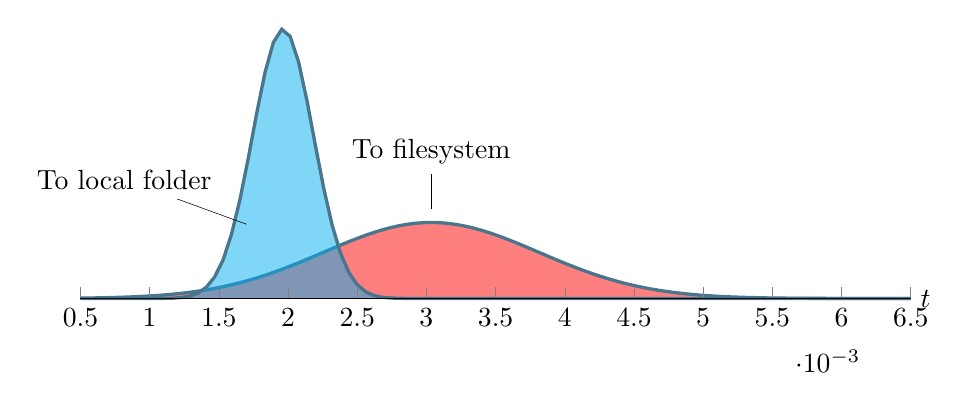
\begin{tikzpicture}
\begin{axis}[
  no markers, domain=0.0005:0.0065, samples=100,
  axis lines*=left, xlabel=$t$, ylabel=$1$,
  hide y axis,
  every axis x label/.style={at=(current axis.right of origin),anchor=west},
  height=5cm, width=\textwidth,
  ytick=\empty,
  %xtick={0.253917}, ytick=\empty,
  enlargelimits=false, clip=false, axis on top,
  %grid = major % Will draw full horizontal lines
  ]
  
  \addplot [very thick,cyan!50!black, fill=red, fill opacity=0.5] {512.048 * e^(-823703 * (-0.00303433+x)^2)}; % Test CP
  
  \addplot [very thick,cyan!50!black, fill=cyan, fill opacity=0.5] {1813.75 * e^(-1.03349*10^7*((-0.00196389+x)^2))}; % Base CP
  
\node [
	  coordinate,
	  pin={[pin edge={black}]135:{To local folder}},
 ] at (axis cs:0.0017,500) {};
 
\node [
	coordinate,
	pin={[pin edge={black}]90:{To filesystem}},
] at (axis cs:0.00303433,600) {};
\end{axis}
\end{tikzpicture} % TODO: This is a dummy graph for now
	
	\vspace{0.5cm}
	\noindent \begin{tabular}{l*{4}{c}r}
		& Min & Max & Mean & Std. Div. & \\
		\hline
		Copy to local folder & TODO s & TODO s & \textbf{TODO s} & \textbf{TODO s} &  \\
		Copy to FUSE mountpoint & TODO s & TODO s & \textbf{TODO s} & \textbf{TODO s} &  \\
		Distance           & +TODO s & +TODO s & \textbf{+TODO s} & \textbf{+TODO s} & \\
	\end{tabular}

	\vspace{0.25cm}
	
	\subsection{Analysis}
	% TODO
\end{document}
